\documentclass[a4paper,11pt]{article}
\usepackage{commonpackages}

\usepackage{xcolor}
\definecolor{mybackcolor}{rgb}{0.98,0.98,0.98}

\lstset{language=HTML, basicstyle={\small\ttfamily}, keywordstyle=\color{blue}, identifierstyle=\color{darkgray}, stringstyle=\color{brown}, backgroundcolor=\color{mybackcolor}, numbers=left}

\begin{document}
\title{CSS}
\date{}
\maketitle

\section{Définition du format CSS}
Le langage \textbf{CSS} (Cascading Style Sheet en français feuilles de style en cascade) permet de mettre en forme les documents HTML. Il permet notamment de modifier la police, la couleur, la taille et l'emplacement du contenu.\\
CSS est un langage basé sur des règles: il permet de définir des règles de style pour un type d'élément donné, par exemple les titres principaux <h1></h1> ou les paragraphes <p></p>

\subsection{Structure du code CSS}
\begin{tabular}{l l}
sélecteur \{ & La règle commence par un sélecteur\\
\quad propriété1: valeur1;  & à chaque propriété correspond une valeur est attribuée\\
\quad propriété2: valeur2; & \\
\}& \\
\end{tabular}

\begin{multicols}{2}
\begin{verbatim}{css}
h1 {
  color: green;
  text-align: center;
}
\end{verbatim}\par
Défini le style du titre principal\\
La couleur du texte est verte\\
L'alignement du texte est centré\\
\end{multicols}

% \begin{multicols}{2}
% \includegraphics[width=0.35\textwidth]{css2}\par
% Défini le style des paragraphes\\
% La police utilisée est verdana\\
% La taille de la police est 20 pixels\\
% \end{multicols}

% \subsection{Référencement - Balise <link \dots>}
% Comme le ficher HTML (.html) et le fichier CSS (.css) sont deux fichiers distincts, il faut ajouter au document HTML une référence au fichier CSS. Cela se fait dans le <head> du document HTML avec la balise <link>.
% La balise <link> a deux attributs: rel (précise à quoi sert le fichier référencé) et href (chemin d'accès au document):
% \begin{lstlisting}
% <link href="style.css" rel="stylesheet" type="text/css" />
% \end{lstlisting}

% \subsection{Sélecteur}
% Dans ce cours, nous allons travailler sur 3 types de sélecteurs:
% \begin{itemize}
% \item sélecteur de type
% \item sélecteur d'identifiant
% \item sélecteur de classe
% \end{itemize}

% \subsubsection{Sélecteur de type}
% Le sélecteur de type permet d'appliquer un style à toutes les balises de même type (h1, h2, p, \dots).
% Il est de la forme: \par
% \includegraphics[width=0.4\textwidth]{css1}\par
% Ce style s'appliquera au contenu des balises <h1>…</h1>

% \subsubsection{Sélecteur d'identifiant}
% Le sélecteur d'identifiant permet d'appliquer un style à un élément précis. Pour cela, il faut ajouter un nouvel attribut id à la balise HTML concernée.\par

% \begin{tabular}{|>{\centering}p{7.5cm}| >{\centering}p{7.5cm}|}
% \hline
% \centering Fichier HTML & Fichier CSS\tabularnewline
% \hline
% \includegraphics[width=0.43\textwidth]{html3} & \includegraphics[width=0.4\textwidth]{css3}\tabularnewline
% \hline
% \end{tabular}\par
% Ce style s'appliquera qu'aux balises dont l'id est "intro".

% \subsubsection{Sélecteur par classe}
% Le sélecteur de classe permet d'appliquer un style à plusieurs éléments qui appartiennent à un même classe (groupe). Pour cela, il faut ajouter un nouvel attribut class à la balise HTML concernée.\par

% \begin{tabular}{|>{\centering}p{7.5cm}| >{\centering}p{7.5cm}|}
% \hline
% \centering Fichier HTML & Fichier CSS\tabularnewline
% \hline
% \includegraphics[width=0.43\textwidth]{html4} & \includegraphics[width=0.4\textwidth]{css4}\tabularnewline
% \hline
% \end{tabular}\par
% Ce style s'appliquera qu'aux balises dont la class est "intro".

% Tuto: \url{https://developer.mozilla.org/fr/docs/Learn/Getting_started_with_the_web/CSS_basics}

% \exo
% But: Appliquer un fichier CSS au document index.html.
% \begin{enumerate}[label=\arabic*)]
% \item Sur Moodle, télécharger le document \textbf{style.css}.
% \item Sauvegarder ce document sur OneDrive dans le dossier informatique.
% \item Sur replit.com, il faut remplacer le fichier style.css par celui que vous venez de télécharger:
% \begin{enumerate}
%   \item Effacer le fichier \textbf{style.css} déjà présent.
%   \item Télécharger votre fichier en cliquant sur les 3 points verticaux et en séléctionnant \textbf{Upload file}. Choisir le fichier \textbf{ style.css} que vous avez sauvergarder sur votre OneDrive.
% \end{enumerate}
% \item Ajouter le référencement à la page \textbf{style.css} dans le <head> du document \textbf{index.html}. (cf. 4.2)
% \item Appuyer sur le bouton \textbf{Run}.
% \end{enumerate}

% \exo
% \begin{enumerate}[label=\arabic*)]
% \item Qu'est-ce qui a changé?
% \item Cliquer sur \textbf{style.css} pour que le document s'afficher et essayer de le comprendre.
% \begin{enumerate}
%   \item À quels éléments s'appliquent les différentes propriétés?
%   \item Quelle est la différence entre h1{\dots} et \#source{\dots}? Quand va-t-on utiliser le deuxième?
% \end{enumerate}
% \item Vous allez maintenant modifier cette page (pour valider une modification, appuyer sur \textbf{Run}):
% \begin{enumerate}
%   \item Modifier la couleur des titres et des sous-titres. Vous pouvez utiliser les noms en anglais ou le code RGB.\\
%   Liste des couleurs: \url{https://www.rapidtables.com/web/color/RGB_Color.html}
%   \item Modifier la police de caractère (font) des titres (pas des sous-titres) en  "fantasy".
%   \item Modifier la couleur de fond de la page HTML.
%   \item Ajouter une couleur de fond aux titres et aux sous-titres.
%   \item Modifier le code pour que toutes les sources s'affichent en gris foncé. (Il faut utiliser un sélecteur de classe.)
% \end{enumerate}
% \end{enumerate}

% \newpage

% \subsection{Conteneurs <div>}
% \begin{multicols}{2}
% Un conteneur est un élément qui contient plusieurs éléments et qui est défini comme un bloc.
% Il est défini en HTML par la balise <div> \dots </div>. Dans le fichier CSS, il est possible de définir différentes propriétés d'un bloc, comme la hauteur (height), la largeur (width), la marge intérieure (padding), la marge extérieure (margin) ou la bordure (border).
% 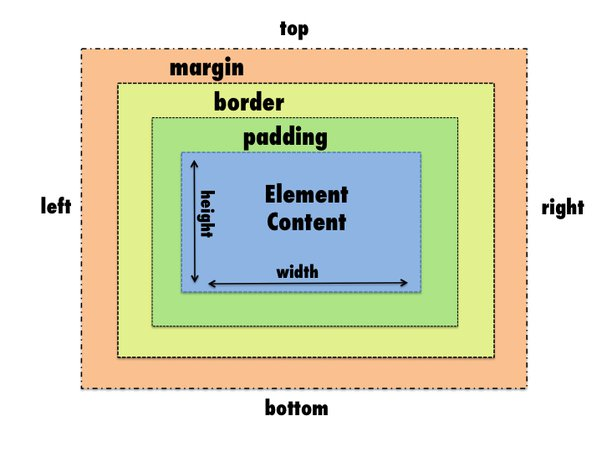
\includegraphics[width= 0.45\textwidth]{conteneur}
% \end{multicols}

% \begin{tabular}{|>{\centering}p{7.5cm}| >{\centering}p{7.5cm}|}
% \hline
% \centering Fichier HTML & Fichier CSS\tabularnewline
% \hline
% \includegraphics[width=0.5\textwidth]{html5} & \includegraphics[width=0.4\textwidth]{css5}\tabularnewline
% \hline
% \end{tabular}\par
% Tuto: \url{https://developer.mozilla.org/fr/docs/Web/HTML/Element/div}

% \exo
% À vous de jouer. Réfléchir à la structure de votre site internet:
% \begin{enumerate}
% \item Quelles seront les différentes pages?\\
% Sur replit.com, il est nécessaire que la première page de votre site s'appelle \textbf{index.html}. Vous pouvez en créer d'autres et les référencer avec des liens pour pouvoir naviguer entre les différentes pages de votre site.
% \item Quel sera le style de votre site? Pouvez-vous le réaliser avec les outils vus en classe? Sinon rechercher sur internet comment faire.
% \end{enumerate}

% \section{Tutos}
% Tuto pour HTML: \url{https://developer.mozilla.org/fr/docs/Web/HTML}\par
% Tuto pour CSS: \url{https://developer.mozilla.org/fr/docs/Web/CSS}\par
% Tuto en anglais: \url{https://www.w3schools.com/ }

% \vfill
% \renewcommand{\refname}{Références}
% \begin{thebibliography}{9}
% \bibitem{mozilla} https://developer.mozilla.org/fr/docs/Web
% \bibitem{Marro} https://www.wiki.mathematix.ch/doku.php (cours de R. Lehmann et C. Marro)
% \bibitem{Schaller} https://www.info.we-tea.ch/doku.php (cours de G. Schaller)
% \bibitem{Livre} GREGOIRE, Sylvie; MOUSSIER, Pascal: \emph{Sciences Numériques et Technologiques 2\textsuperscript{de}}, Paris: Nathan, 2019.
% \end{thebibliography}


% \newpage
% \section{Solution des exercices}

% \lstset{identifierstyle=\color{black}, commentstyle=\color{gray}}

% \sol
% Correction directement sur Moodle.

% \sol
% Marche à suivre.

% \sol
% 1) Fichier index.htlm
% \begin{lstlisting}
% <!DOCTYPE html> <!-- indique le genre de document au browser -->
% <html>
%   <head> <!-- métadonnées de la page et le titre de l'onglet -->
%     <meta charset="utf-8">
%     <title>Nom de la page</title>
%   </head>
%   <body> <!-- partie qui sera affichée -->
%     <h1>Le collège du Sud</h1> <!-- titre principal -->
%     <!-- 1er paragraphe -->
%     <p>Voici ma première page Web sur le collège du Sud!</p>
%     <h2>Présentation</h2> <!-- Sous-titre -->
%     <!-- 2e paragraphe -->
%     <p>
%     Le Collège du Sud est un établissement fribourgeois du
%     secondaire du 2e degré. Il offre actuellement 3 filières
%     d’études : un gymnase, une école de commerce et une école
%     de culture générale. Il reçoit des étudiant-e-s de 16 à 20 ans,
%     qui proviennent essentiellement des districts de la Gruyère
%     et de la Veveyse, mais aussi de la Glâne.</p>
%     <!-- Ajout d'une image -->
%     <p id="source">Source:
%     <a href="https://collegedusud.ch/presentation/" target="_blank">
%     Site internet du collège du Sud</a>
%     <p/>
%     <h2>Mes cours</h2> <!-- Sous-titre -->
%       <ul> <!-- liste non numérotée -->
%         <li>Français</li>
%         <li>Allemand</li>
%         <li>Anglais</li>
%         <li>Maths</li>
%       </ul>

%     </body>
% </html>
% \end{lstlisting}
% 2) Fichier index.html modifié
% \begin{lstlisting}
% <!DOCTYPE html>
% <html>
%   <head>
%     <meta charset="utf-8">
%     <title>Nom de la page</title>
%   </head>
%   <body>
%     <h1>Le collège Sainte-Croix</h1>
%     <p>Voici ma première page Web sur le collège Sainte-Croix!</p>
%     <h2>Présentation</h2>
%     <p>
%     Le Collège Sainte-Croix est un établissement fribourgeois
%     du secondaire du 2e degré. C'est un gymnase en ville de Fribourg
%     qui permet de faire une maturité en français, en allemand ou un
%     mixte des deux langues. Il reçoit des étudiant-e-s de 16 à 20 ans.
%     </p>
%     <p id="source">Source:
%     <a href="https://new.cscfr.ch/index.php/fr/" target="_blank">
%     Site internet du collège Sainte-Croix</a><p/>
%     <h2>Mes cours</h2>
%     <ol>
%       <li>Français</li>
%       <li>Allemand</li>
%       <li>Anglais</li>
%       <li>Maths</li>
%       <li>Économie et droit</li>
%       <li>Biologie</li>
%       <li>...</li>
%     </ol>
%     <h2>Ma classe</h2>
%     <p>
%     Je fais partie de la classe 1F... qui est une classe qui ...
%     <p/>
%     <img src = "images/STX.jpg" width ="600" height ="400"><br/>
%     Source:
%     <a href="https://new.cscfr.ch/index.php/fr/notre-college/nos-batiments/">
%     https://new.cscfr.ch/index.php/fr/notre-college/nos-batiments/</a>
%   </body>
% </html>
% \end{lstlisting}

% \sol
% Il faut ajouter la ligne suivante dans le <head></head> du fichier html:
% \begin{lstlisting}
% <link href ="style.css" rel="stylesheet" type ="text/css" />
% \end{lstlisting}

% \sol
% Ce qui a changé:
% \begin{enumerate}
% \item Le titre est en rose et les sous-titres sont en violet.
% \item La couleur de fond de la page est gris.
% \item Le type de police et la taille sont différents.
% \item Le mot "source" dans la partie présentation est en italique.
% \end{enumerate}
% h1 sera appliqué à tous les titres. \#source sera appliqué seulement à l'élément dont l'identifiant sera \#source. Si nous souhaitons appliquer un style sur plusieurs éléments, il faut utiliser un sélecteur de classe.\par
% \includegraphics[width=0.4\textwidth]{cssex5}\par
% Ne pas oublier de changer, dans le fichier html, les sources avec un sélecteur par classe pour pouvoir l'utiliser à chaque source:
% \begin{lstlisting}
% ...
%     <p class="source">Source:
%     <a href="https://new.cscfr.ch/index.php/fr/" target="_blank">
%     Site internet du collège Sainte-Croix</a><p/>
% ...
%     <p class="source">Source:
%     <a href="https://new.cscfr.ch/index.php/fr/notre-college/nos-batiments/">
%     https://new.cscfr.ch/index.php/fr/notre-college/nos-batiments/</a>
% ...
% \end{lstlisting}
\end{document}
